\chapter{Simulado 1}
\markboth{Simulado 1}{}

\num{1} Veja o animal que Bia encontrou na praia.

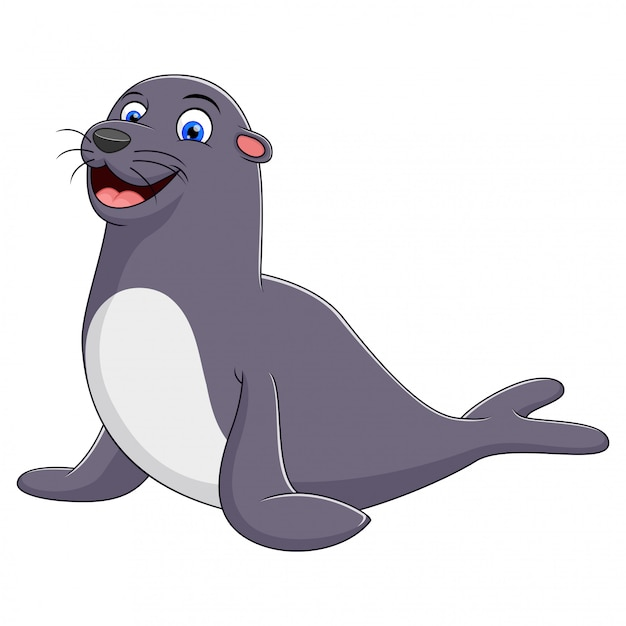
\includegraphics[width=2.16528in,height=1.72778in]{media/image139.jpeg}

%Disponível em:https://www.freepik.com/premium-vector/seal-cartoon-isolated\_6122224.htm\#query=FOCA\&position=35\&from\_view=search\&track=sph. Acesso 07 mar. 2023.

A palavra que começa com a mesma letra inicial do nome desse animal é

\begin{escolha}
\item Vaca.

\item Fada.

\item Toca.

\item Doce.
\end{escolha}

\num{2} Observe o utensílio que Paula ganhou para sua cozinha.

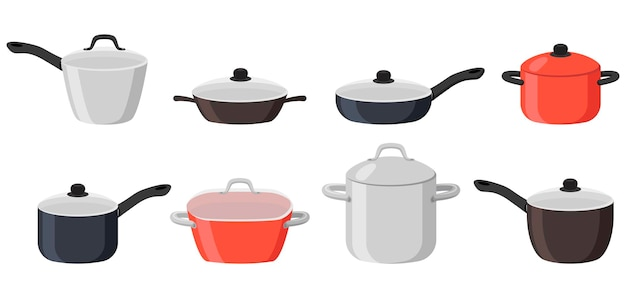
\includegraphics[width=1.22222in,height=1.11389in]{media/image19.jpeg}

%https://www.freepik.com/free-vector/frying-pans-saucepans-cartoon-illustration-set-metal-cooking-pots-with-lid-different-sizes-stainless-utensils-making-soup-boiling-water-household-kitchen-concept\_26921753.htm\#query=PANELA\&position=0\&from\_view=search\&track=sph

A palavra cujo som inicial é igual ao da primeira sílaba do nome do utensílio é

\begin{escolha}
\item Papagaio.

\item Banana.

\item Janela.

\item Peteca.
\end{escolha}

\num{3} Veja o móvel novo que Dona Lili comprou na loja do seu bairro.

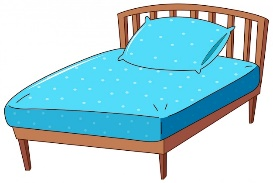
\includegraphics[width=1.22293in,height=0.81839in]{media/image140.jpeg}

%https://www.freepik.com/free-vector/bed-with-blue-pillow-sheet\_2204447.htm\#page=2\&query=CAMA\&position=15\&from\_view=search\&track=sph\#page=2\&query=C\&from\_query=undefined\&position=0\&from\_view=search\&track=sph

A palavra que começa com a mesma sílaba inicial do nome do móvel que Dona Lili comprou é

\begin{escolha}
\item Cenoura.

\item Cinema.

\item Cavalo.

\item Cisne.
\end{escolha}

\num{4} Veja o alimento preferido do ratinho Fifi.

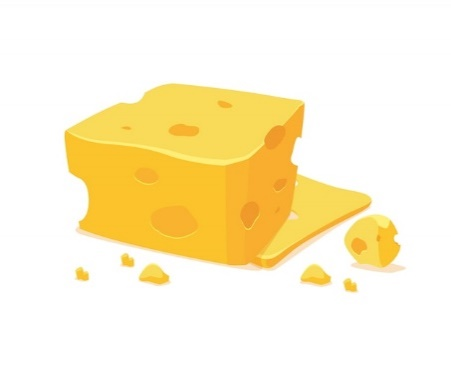
\includegraphics[width=1.56736in,height=0.94861in]{media/image141.jpeg}

%Disponível em:https://www.freepik.com/premium-vector/cheese-slices-cartoon-style\_6537367.htm?query=QUEIJO\#from\_view=detail\_alsolike Acesso em: 08 mar. 2023.

A escrita correta do nome do alimento de fifi é

\begin{escolha}
\item Qeijo.

\item Cueijo.

\item Queijo.

\item Cuijo.
\end{escolha}

\num{5} Observe o animal preferido de Gustavo.

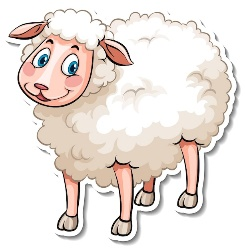
\includegraphics[width=1.11458in,height=1.13889in]{media/image142.jpeg}

%Disponível em:https://www.freepik.com/free-vector/sheep-farm-animal-cartoon-sticker\_21849763.htm\#query=OVELHA\&position=41\&from\_view=search\&track=sph.acesso em 08 mar. 2023.

A separação silábica do nome animal de Gustavo é

\begin{escolha}
\item O -- ve -- lha

\item O -- v -- e -- lha.

\item O -- ve -- l -- ha.

\item Ve -- lh -- a.
\end{escolha}

\num{6} Observe a fruta de que Felipe mais gosta.

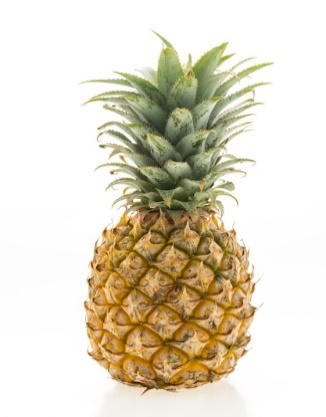
\includegraphics[width=0.94236in,height=1.64306in]{media/image143.jpeg}

%Disponível em:https://www.freepik.com/free-photo/pineapple-fruit\_1123681.htm\#query=ABACAXI\&position=4\&from\_view=search\&track=sph. Acesso 08 mar. 2023.

Qual palavra apresenta as mesmas sílabas iniciais da fruta preferida de Felipe?

\begin{escolha}
\item Goiaba.

\item Banana.

\item Abacate.

\item Graviola.
\end{escolha}

\num{7} Veja a palavra que Artur tirou em um sorteio para ganhar um instrumento musical.

\textbf{BATERIA}

A palavra cuja sílaba inicial é a mesma do nome do instrumento que ele tirou é

\begin{escolha}
\item Pedra.

\item Batata.

\item Morango.

\item Computador.
\end{escolha}

\num{8} Obseve a imagem:

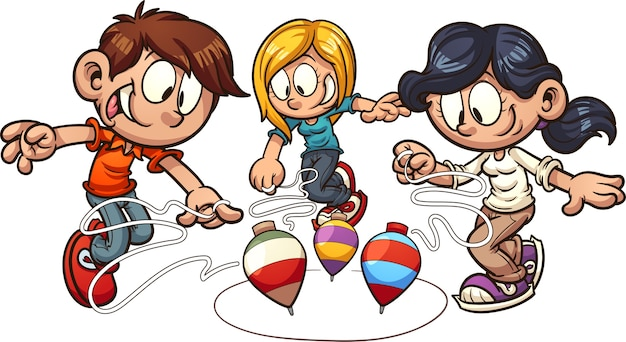
\includegraphics[width=3.05095in,height=1.66841in]{media/image144.jpeg}

%Disponível em: \url{https://br.freepik.com/vetores-premium/piao-criancas_2502255.htm}. Acesso 08 mar. 2023.

A frase que representa a imagem é

\begin{escolha}
\item As crianças brincam com pião.

\item As crianças brincam de pipa.

\item A criança brinca com o pião.

\item O pião das crianças sumiu.
\end{escolha}

\num{9}

\begin{verse}
\textbf{A barata}

A barata diz que tem\\
Sete saias de filó.\\
É mentira da barata\\
Ela tem é uma só.

ah! ah! ah!\\
oh! oh! oh!\\
Ela tem é uma só.

A barata diz que tem\\
Sete saias de balão.\\
É mentira ela não tem\\
Nem dinheiro pro sabão.

Ah! ah! ah!\\
Oh! oh! oh!\\
Nem dinheiro pro sabão.

A barata diz que tem\\
Um sapato de fivela.\\
É mentira da barata\\
O sapato é da mãe dela.

Ah! ah! ah!\\
Oh! oh! oh!\\
O sapato é da mãe dela.
\end{verse}

\fonte{Disponível em:
http://www.dominiopublico.gov.br/download/texto/me000588.pdf Acesso 8
mar. 2023.}

O que a barata tem em somente uma quantidade?

\begin{escolha}
\item Saia de filó

\item Saia de balão.

\item Sapato de fivela.

\item Dinheiro pra sabão.
\end{escolha}

\num{10} Bianca vai fazer um bolo de milho para receber sua amiga em sua casa.

O texto que ela deve usar para fazer o bolo é

\begin{escolha}
\item Uma agenda.

\item Um convite.

\item Um verbete.

\item Uma receita.
\end{escolha}

\num{11} Leia o anúncio:

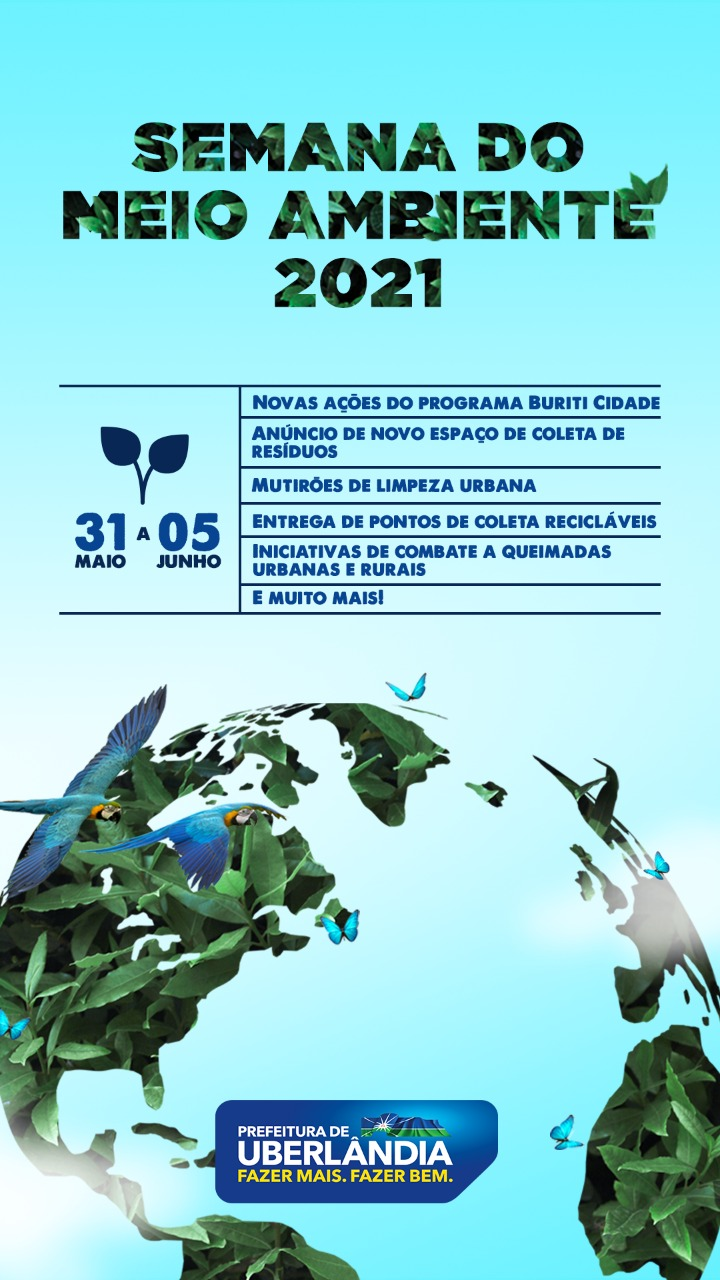
\includegraphics[width=3.12674in,height=4.31210in]{media/image145.jpeg}

%Disponível em \url{https://www.uberlandia.mg.gov.br/2021/05/28/prefeitura-promove-acoes-e-realiza-anuncios-na-semana-do-meio-ambiente-2021/} Acesso 11 mar. 2023

Esse texto serve para

\begin{escolha}
\item Ensinar.

\item Divertir.

\item Alertar.

\item Anunciar.
\end{escolha}

\num{12}

\begin{verse}
\textbf{MARINHEIRO SÓ}

Marinheiro só\\
Lá vem, lá vem\\
Marinheiro só\\
Todo de branco\\
Marinheiro só\\
Com seu bonezinho.

\end{verse}

\fonte{Disponível
em: http://www.dominiopublico.gov.br/download/texto/me000588.pdf.
Acesso 08 mar. 2023.}

Quem anda todo de branco?

\begin{escolha}
\item O boné do marinheiro.

\item O navio do marinheiro.

\item O marinheiro.

\item O amigo do marinheiro.
\end{escolha}

\num{13} Leia:

\begin{verse}
Meio-dia
Macaco assobia
Panela no fogo
Barriga vazia.
\end{verse}

\fonte{Disponível
em: http://www.dominiopublico.gov.br/download/texto/me000588.pdf. Acesso em:
08 mar. 2023.}

A barriga está vazia porque

\begin{escolha}
\item O fogo tinha apagado.

\item A comida queimou na panela.

\item O macaco tinha comido tudo.

\item Porque estava na hora do almoço.
\end{escolha}


\num{14}

%Paulo: inserir a figura disponível no endereço https://br.freepik.com/vetores-gratis/pessoa-dormir-cama-fundo_4434144.htm#query=sleeping%20comic%20book&position=4&from_view=search&track=robertav1_2_sidr

A onomatopeia zzzzz que aparece no quadrinho mostra que

\begin{escolha}
\item O menino está gritando.

\item O menino está dormindo.

\item O menino está chorando.

\item O menino está sussurrando.
\end{escolha}

\num{15} Leia o quadrinho.

%Paulo: inserir imagem disponível no endereço https://br.freepik.com/vetores-gratis/personagem-de-empresaria-muito-zangada-ilustracoes-de-design-vetorial-de-estilo-doodle-desenhado-a-mao_25864757.htm#query=angry%20woman%20drawing&position=4&from_view=search&track=robertav1_2_sidr

A expressão facial da mulher mostra que ela está

\begin{escolha}
\item Alegre.

\item Sussurrando.

\item Chorando.

\item Nervosa.
\end{escolha}

\num{16}

\textbf{O soldadinho de chumbo}

Numa loja de brinquedos havia uma caixa de papelão com
vinte e cinco soldadinhos de chumbo, todos iguaizinhos, pois
haviam sido feitos com o mesmo molde. Apenas um deles
era perneta: como fora o último a ser fundido, faltou chumbo
para completar a outra perna. Mas o soldadinho perneta logo
aprendeu a ficar em pé sobre a única perna e não fazia feio ao
lado dos irmãos.

\fonte{Disponível
em: http://www.dominiopublico.gov.br/download/texto/me001614.pdf.
Acesso 09 mar. 2023.}

O assunto desse texto é

\begin{escolha}
\item A loja de brinquedos.

\item Os soldadinhos de chumbo.

\item O soldadinho diferente.

\item A caixa com os soldadinhos.
\end{escolha}


\chapter{Simulado 2}
\markboth{Simulado 2}{}

\num{1} Observe o presente que Ana ganhou de sua madrinha.

%Paulo: inserir imagem disponível no endereço https://br.freepik.com/vetores-gratis/mao-boneca-pintada_795247.htm#query=boneca%20de%20pano&position=18&from_view=search&track=robertav1_2_sidr

A palavra cuja sílaba inicial é a mesma do nome do presente é

\begin{escolha}
\item Panela.

\item Boné.

\item Vacina.

\item Figo.
\end{escolha}

\num{2} Observe a imagem.

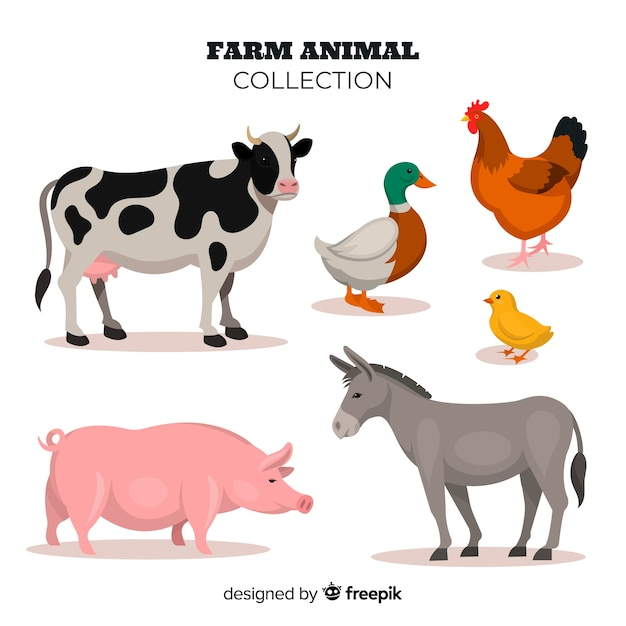
\includegraphics[width=1.10000in,height=0.99236in]{media/image148.jpeg}

%https://www.freepik.com/free-vector/flat-design-farm-animal-collection\_4751955.htm\#query=VACA\&position=1\&from\_view=search\&track=sph

A sílaba inicial do nome desse animal também aparece no início de

\begin{escolha}
\item Vale.

\item Fada.

\item Toca

\item Pato.
\end{escolha}

\num{3} Veja o alimento que o coelhinho Pitoco gosta de comer.

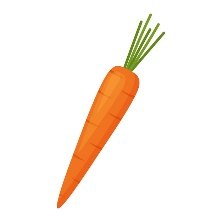
\includegraphics[width=1.01111in,height=1.01111in]{media/image149.jpeg}

%https://www.freepik.com/premium-vector/carrot-vector-illustration\_20583403.htm\#page=2\&query=CENOURA\&position=45\&from\_view=search\&track=sph

A letra inicial do nome do alimento de Pitoco também aparece no início de

\begin{escolha}
\item Fama.

\item Bola.

\item Cinema.

\item Pepino.
\end{escolha}

\num{4} Veja a palavra que Pedro e Tiago formaram no jogo da forca.

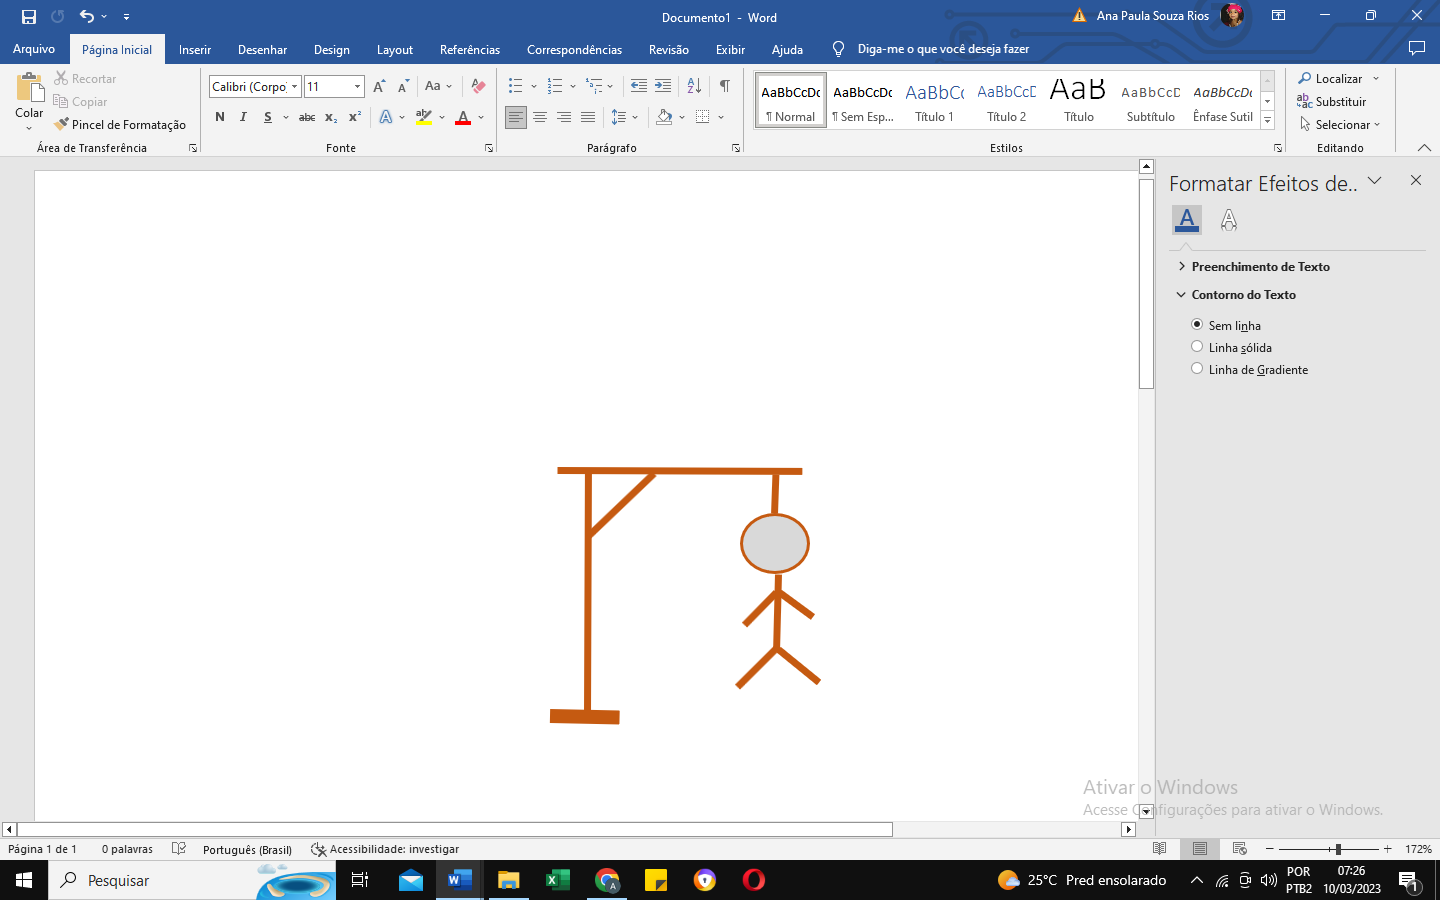
\includegraphics[width=1.50909in,height=1.22355in]{media/image150.png}

Qual letra pode ser usada para formar uma outra palvara?

\begin{escolha}
\item D

\item B

\item F

\item V
\end{escolha}

\num{5} Veja a palavra que Hugo escreveu.

A separação silábica correta da palavra que Hugo escreveu é

\begin{escolha}
\item A -- mo -- ra.

\item Am -- o -- ra.

\item A -- mo -- r -- a.

\item Amo -- r -- a.
\end{escolha}

\num{6} Veja o objeto que Jonas encontrou no rio.

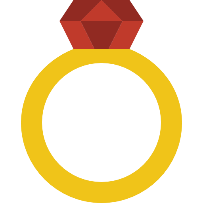
\includegraphics[width=0.92222in,height=0.92222in]{media/image151.png}

%https://www.freepik.com/free-icon/diamond-ring\_14457523.htm?query=ANEL\#from\_view=detail\_alsolike

Assim como o nome do objeto encontrado, qual palavra também é iniciada com vogal?

\begin{escolha}
\item Bala.

\item Apito.

\item Camisa.

\item Panela.
\end{escolha}

\num{7} Observe a fruta que Maria gosta de levar na lancheira.

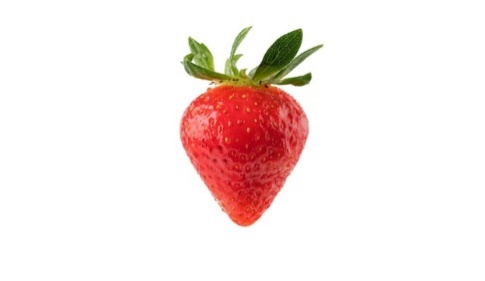
\includegraphics[width=0.73819in,height=0.93750in]{media/image152.jpeg}

%https://www.freepik.com/free-psd/view-ripe-sweet-fruit\_37298510.htm\#query=MORANGO\&position=4\&from\_view=search\&track=sph

A palavra cuja sílaba do meio também é formada pela sequência consoante vogal consoante é

\begin{escolha}
\item Melancia.

\item Formiga.

\item Moqueca.

\item Batom.
\end{escolha}

\num{8} Veja o carro que Mateus dirige levando pessoas para o médico.

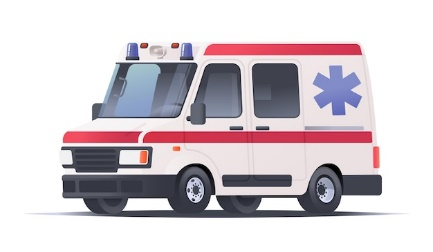
\includegraphics[width=1.54514in,height=0.89444in]{media/image153.jpeg}

%\url{https://www.freepik.com/premium-vector/ambulance-car-isolated-white-background-emergency-vehicle-vector-illustration-cartoon-style_24585760.htm\#query=AMBULANCIA\&position=8\&from_view=search\&track=sph}

A escrita correta do nome desse tipo de carro é

\begin{escolha}
\item Abulância.

\item Ambulâcia.

\item Ambulâmcia.

\item Ambulância.
\end{escolha}

\num{9} Leia a frase.

As crianças estão no rio.

A imagem que representa essa frase é

\begin{escolha}
\item 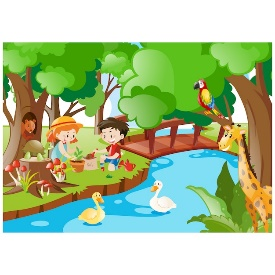
\includegraphics[width=1.25000in,height=0.82361in]{media/image154.jpeg}

\item 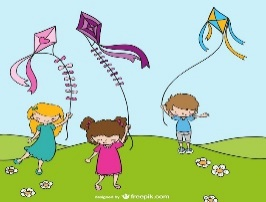
\includegraphics[width=1.21181in,height=0.92014in]{media/image155.jpeg}

\item 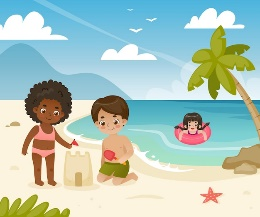
\includegraphics[width=1.18125in,height=0.98472in]{media/image156.jpeg}

\item 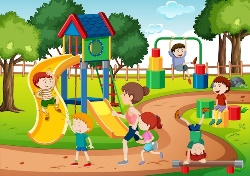
\includegraphics[width=1.13611in,height=0.80208in]{media/image157.jpeg}
\end{escolha}

%https://www.freepik.com/free-vector/nature-landscape-background\_1062401.htm?query=CRIAN\%C3\%87AS\%20BRINCADO\%20NO\%20RIO\#from\_view=detail\_alsolike
%\url{https://www.freepik.com/premium-vector/adorable-children-playing-tropical-beach_29549473.htm?query=CRIAN\%C3\%87AS\%20BRINCADO\%20NA\%20PRAIA\#from_view=detail_alsolike}
%\url{https://br.freepik.com/vetores-gratis/criancas-com-pipas-desenho-animado_753202.htm}
%https://br.freepik.com/vetores-premium/criancas-brincando-na-cena-do-parquinho\_11863217.htm


\num{10} Veja a imagem.

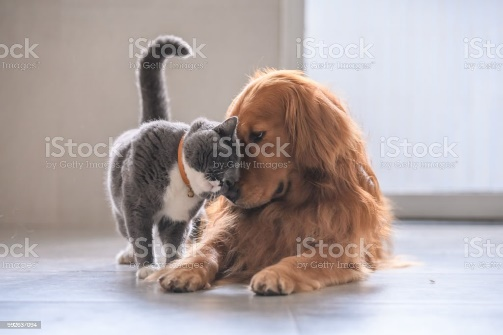
\includegraphics[width=2.27539in,height=1.51515in]{media/image158.jpeg}

%https://www.istockphoto.com/br/foto/gato-de-cabelo-curto-brit\%C3\%A2nico-e-retriever-dourado-gm992637094-268930508?utm\_campaign=srp\_photos\_inline\&utm\_content=https\%3A\%2F\%2Fwww.pexels.com\%2Fprocurar\%2Fgato\%2F\&utm\_medium=affiliate\&utm\_source=pexels\&utm\_term=gato

A frase que representa a imagem é

\begin{escolha}
\item O gato está brigando com o cachorro.

\item O cachoro está latindo para o gato.

\item O cachorro e o gato estão brigando.

\item O gato e o cachorro estão brincando.
\end{escolha}


\num{11} Leia com atenção.

\begin{quote}
\textbf{O rouxinol do imperador}

O palácio do imperador da China era uma das coisas mais
bonitas que existiam no mundo. Construído em mármore
branco, possuía torres de marfim, paredes revestidas com
tecidos de cores variadas e quartos decorados com ouro e
prata. Era realmente uma maravilha!
O jardim também era de enorme beleza; nele cresciam
flores raras e belas. Havia inúmeros rios e lagos, onde
nadavam peixes de todas as espécies e tamanhos.
Para além do jardim, se estendia uma mata, que
chegava até o mar e no interior dela vivia um rouxinol de
canto único.
\end{quote}

\fonte{Disponível em: http://www.dominiopublico.gov.br/download/texto/me001614.pdf Acesso em: 10 mar. 2023.}

Onde vivia o rouxinol?

\begin{escolha}
\item Na mata.

\item No jardim.

\item Nas flores.

\item No palácio.
\end{escolha}


\num{12} Observe o cartaz

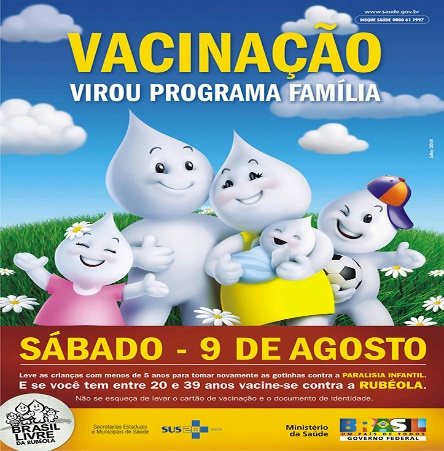
\includegraphics[width=2.01806in,height=2.05069in]{media/image159.jpeg}

Onde é comum encontrarmos esse tipo de cartaz?

\begin{escolha}
\item Nas igrejas.

\item Nas fazendas.

\item Nos locais públicos.

\item Nos parques de diversão.
\end{escolha}

\num{13} Leia:

%
\includegraphics{media/image160.png}
\includegraphics{media/image160.png}

\begin{quote}
\textbf{O lobo e o cão}

Um lobo e um cão se encontraram num caminho. Disse o lobo:

--- Companheiro, você está com ótimo aspecto: gordo, o pêlo lustroso...
Estou até com inveja!

--- Ora, faça como eu --- respondeu o cão. --- Arranje um bom amo.
Eu tenho comida na hora certa, sou bem tratado...
Minha única obrigação é latir à noite, quando aparecem ladrões.
\end{quote}

\fonte{Disponível em
http://www.dominiopublico.gov.br/download/texto/me001614.pdf.
Acesso em: 14 de fev 2023.}

O assunto do texto é:

\begin{escolha}
\item A raiva do lobo pelo cão.

\item A despedida do lobo e o cão.

\item O encontro do cão e o lobo.

\item O convite que o cão fez para o lobo.
\end{escolha}


\num{14}

\begin{verse}
Lá vai a bola\\
Girar na roda\\
Passear depressa\\
E sem demora\\
E se no fim\\
Desta canção\\
Você estiver\\
Com a bola na mão\\
Depressa pule fora.
\end{verse}

\fonte{Disponível
em: http://www.dominiopublico.gov.br/download/texto/me000588.pdf.
Acesso 12 mar. 2023.}

O que acontece com quem ficar com a bola na mão?

\begin{escolha}
\item Sai da brincadeira.

\item Pula de um pé só.

\item Gira na roda.

\item Ganha a bola.
\end{escolha}


\num{15} Veja a imagem


\includegraphics[width=2.09091in,height=1.52916in]{media/image161.jpeg}

%https://br.freepik.com/vetores-gratis/um-modelo-de-adesivo-de-um-personagem-de-desenho-animado-de-gato\_18755484.htm\#page=2\&query=cama\%20de\%20gato\&position=31\&from\_view=keyword\&track=ais

A onomatopeia zzzzz que aparece na imagem mostra que o gatinho está

\begin{escolha}
\item Miando.

\item Agitado.

\item Brincando.

\item Dormindo.
\end{escolha}

\num{16} Observe a imagem.

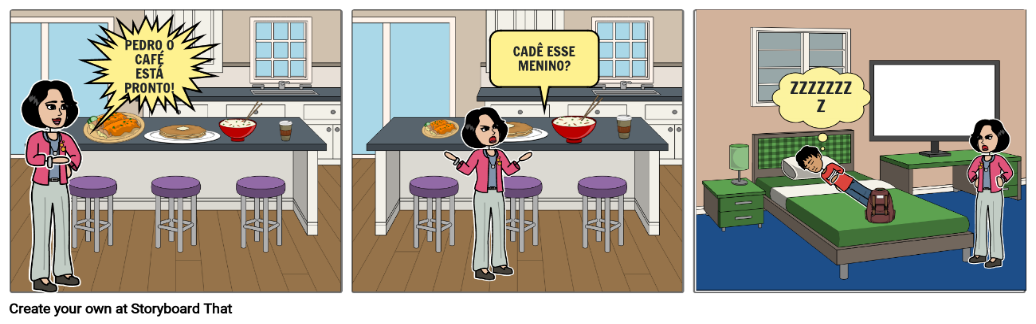
\includegraphics[width=1.57333in,height=1.45456in]{media/image162.png}

%Paulo: inserir imagem disponível no endereço https://br.freepik.com/fotos-gratis/retrato-de-menino-com-raiva_24749739.htm#query=screaming%20boy&position=31&from_view=search&track=robertav1_2_sidr

A imagem indica que a garoto está

\begin{escolha}
\item Chorando.

\item Pulando.

\item Gritando.

\item Dormindo.
\end{escolha}

\chapter{Simulado 3}
\markboth{Simulado 3}{}

\num{1} Veja o que o que Marcos ganhou da sua tia.

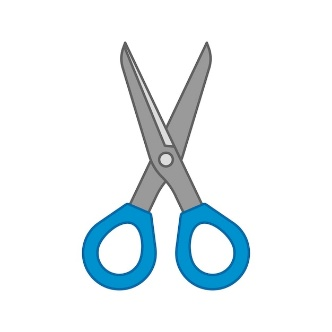
\includegraphics[width=0.92708in,height=1.18125in]{media/image163.jpeg}

%\url{https://www.freepik.com/premium-vector/scissor-isolated-white-background-vector-illustration_27711839.htm\#page=2\&query=TESOURA\&position=23\&from_view=search\&track=sph}

A palavra que começa com o mesmo som da letra inicial do objeto que
Marcos ganhou é

\begin{escolha}
\item Ferro.

\item Tomate.

\item Dominó.

\item Vassoura.
\end{escolha}

\num{2} Veja a palavra que Ana escreveu.

%Paulo: colocar a palavra VILA em um quadro.

A primeira letra da palavra também aparece no início de 

\begin{escolha}
\item Fila.

\item Bala.

\item Vela.

\item Bife.
\end{escolha}

\num{3} Veja o pássaro que pousou na árvore.

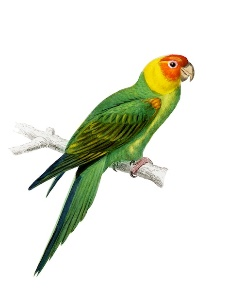
\includegraphics[width=1.08542in,height=1.27222in]{media/image165.jpeg}

%https://www.freepik.com/free-vector/psittacus-eximius-illustrated\_3098865.htm\#query=periquito\&position=29\&from\_view=search\&track=sph

A escrita correta do nome desse pássaro é

\begin{escolha}
\item Perequto.

\item Pericuito.

\item Periquito.

\item Periqito.
\end{escolha}

\num{4} Veja a palavra que as amigas descobriram no jogo da forca.

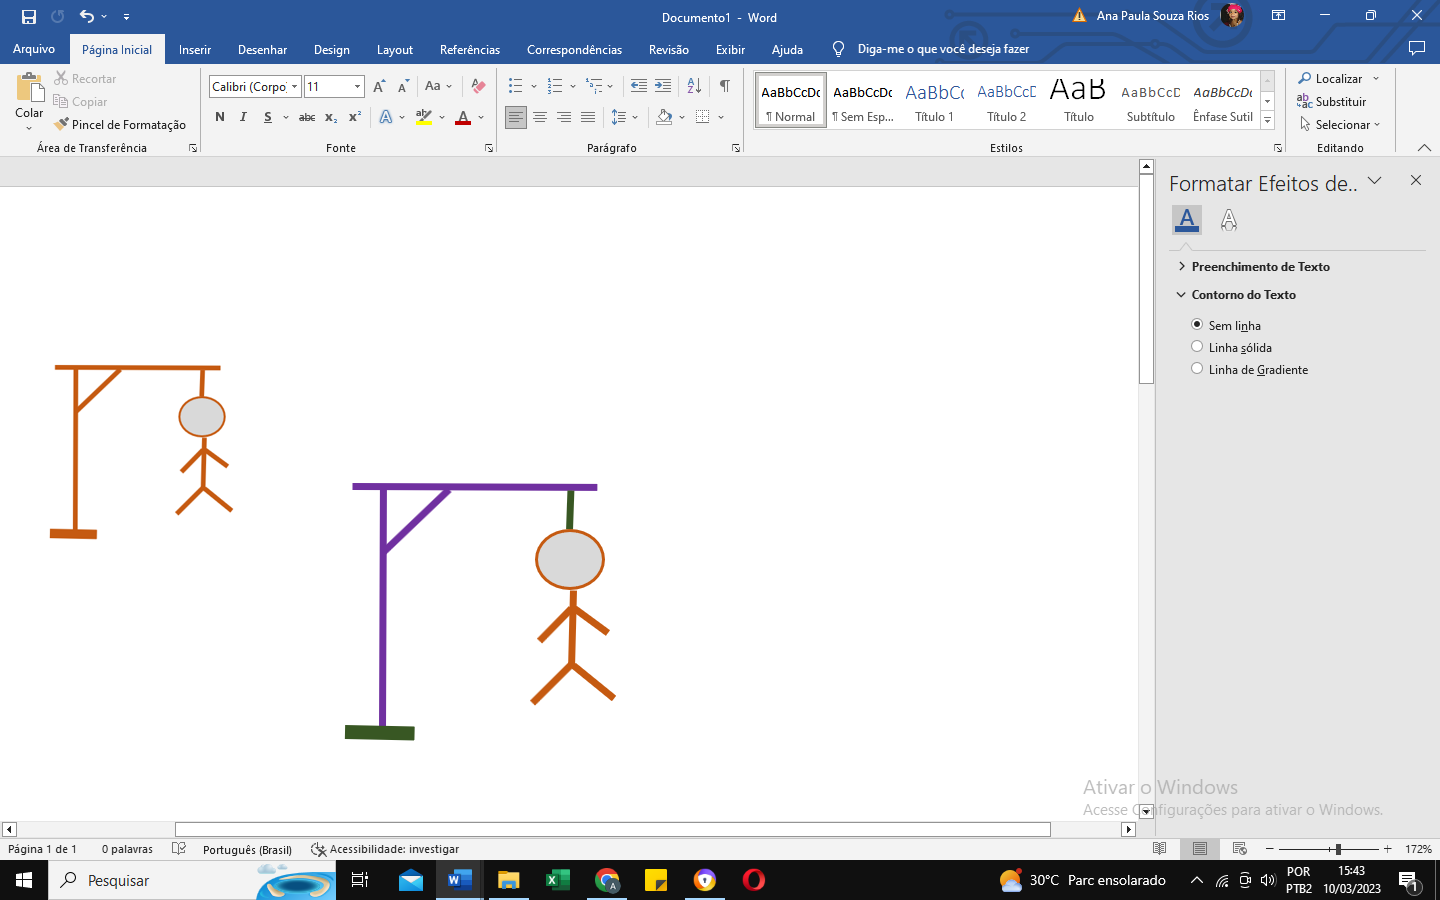
\includegraphics[width=1.24236in,height=1.17500in]{media/image166.png}

A palavra que começa com a mesma sílaba da palavra que elas descobriram é

\begin{escolha}
\item Cachorro.

\item Cinema.

\item Cebola.

\item Comida.
\end{escolha}

\num{5} Veja a palavra que Lívia leu para sua professora.

Assim como a palavra escrita, a sequência consoante vogal consoante também é encontrada na sílaba medial de

\begin{escolha}
\item Banco.

\item Tapete.

\item Macaco.

\item Morango.
\end{escolha}

\num{6} Observe a figura.

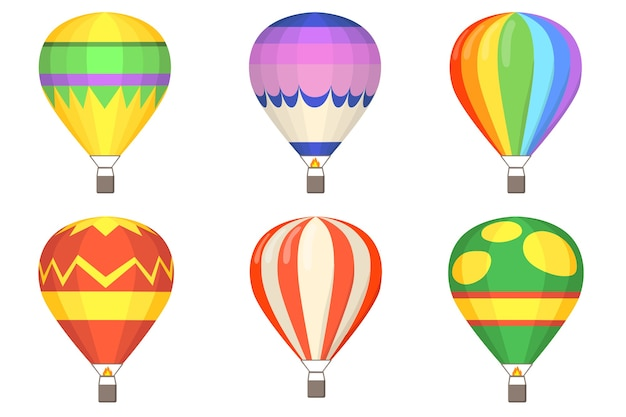
\includegraphics[width=1.22569in,height=1.65417in]{media/image167.jpeg}

%\url{https://www.freepik.com/free-vector/hot-air-balloons-flat-illustration-set-cartoon-colorful-balloons-with-baskets-isolated-vector-illustration-collection-flight-sky-summer-concept_10613127.htm\#page=2\&query=bal\%C3\%A3o\&position=16\&from_view=search\&track=sph}

A escrita correta do nome da figura é

\begin{escolha}
\item Balao.

\item Dalão.

\item Balão.

\item Dalaõ.
\end{escolha}


\num{7} Veja o mimo que Tália ganhou de sua amiga.

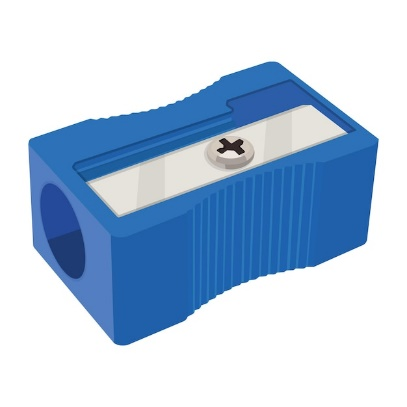
\includegraphics[width=1.67273in,height=1.37251in]{media/image168.jpeg}

%\url{https://www.freepik.com/premium-vector/blue-sharpener-isolated-white-background_25468883.htm\#query=sharpener\&from_query=APONTADOR\&position=12\&from_view=search\&track=sph}

A separação silábica do nome da figura é

\begin{escolha}
\item Ap -- on -- ta -dor.

\item A -- pon -- ta -- dor.

\item Apo -- n -- ta -- do -- r.

\item A -- pon -- t -- ador
\end{escolha}

\num{8} Observe a imagem.

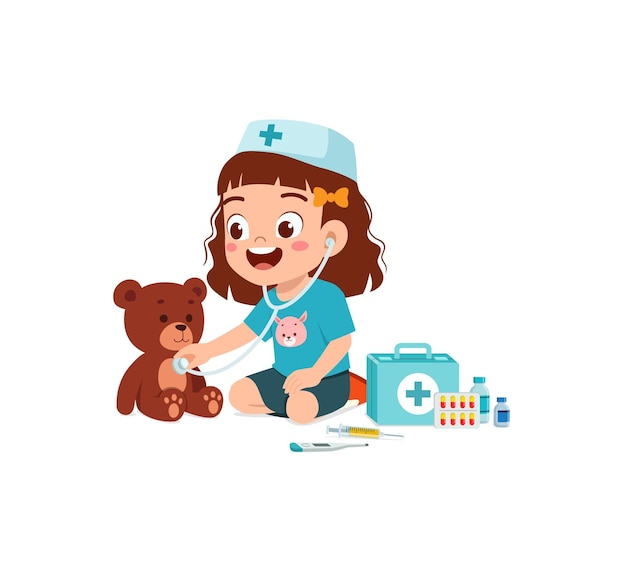
\includegraphics[width=1.87273in,height=1.62645in]{media/image169.jpeg}

%https://www.freepik.com/premium-vector/little-kid-wearing-doctor-costume-play\_31997682.htm\#from\_view=detail\_author

A frase que representa o que está acontecendo na imagem é

\begin{escolha}
\item A menina não gosta do urso.

\item A menina brinca de boneca.

\item A menina brinca de médica.

\item A menina vende os brinquedos.
\end{escolha}

\num{9} Leia a receita:

\textbf{Ingredientes:}\\
1 prato raso de rúcula\\
1 prato raso de alface americana\\
1 prato raso de alface roxa\\
2 xícaras de tomate cereja\\
4 nozes picadas\\
4 castanhas do brasil picadas\\
6 damascos secos picados

\textbf{Preparo:}\\
misturar todos os ingredientes em uma saladeira e servir.

\fonte{Disponível
em: https://www.flickr.com/photos/cbnsp/8263487889/in/photostream/.
Acesso 03 mar. 2023.}

Quantos damascos serão usados para preparar a receita?

\begin{escolha}
\item Um

\item Dois

\item Seis

\item Quatro
\end{escolha}


\num{10} Marta irá ao mercado para fazer as compras da semana.

O texto que ela vai usar para organizar os itens da compra é

\begin{escolha}
\item uma lista.

\item uma agenda.

\item um bilhete.

\item um anúncio.
\end{escolha}

\num{11}

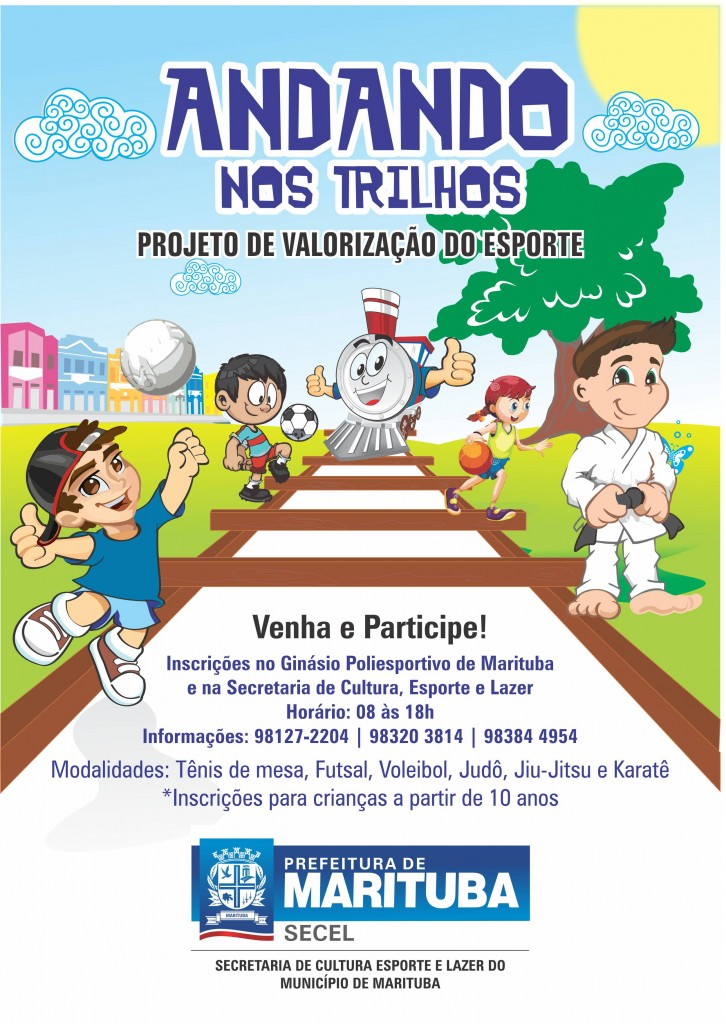
\includegraphics[width=3.11515in,height=2.97237in]{media/image170.jpeg}

%\url{https://marituba.pa.gov.br/site/andando-nos-trilhos/\#prettyPhoto/1/.Acesso} 11 mar. 2023.

Esse anúncio é destinado

\begin{escolha}
\item aos idosos.

\item aos adultos.

\item às crianças.

\item às mulheres.
\end{escolha}


\num{12} Veja o cartaz

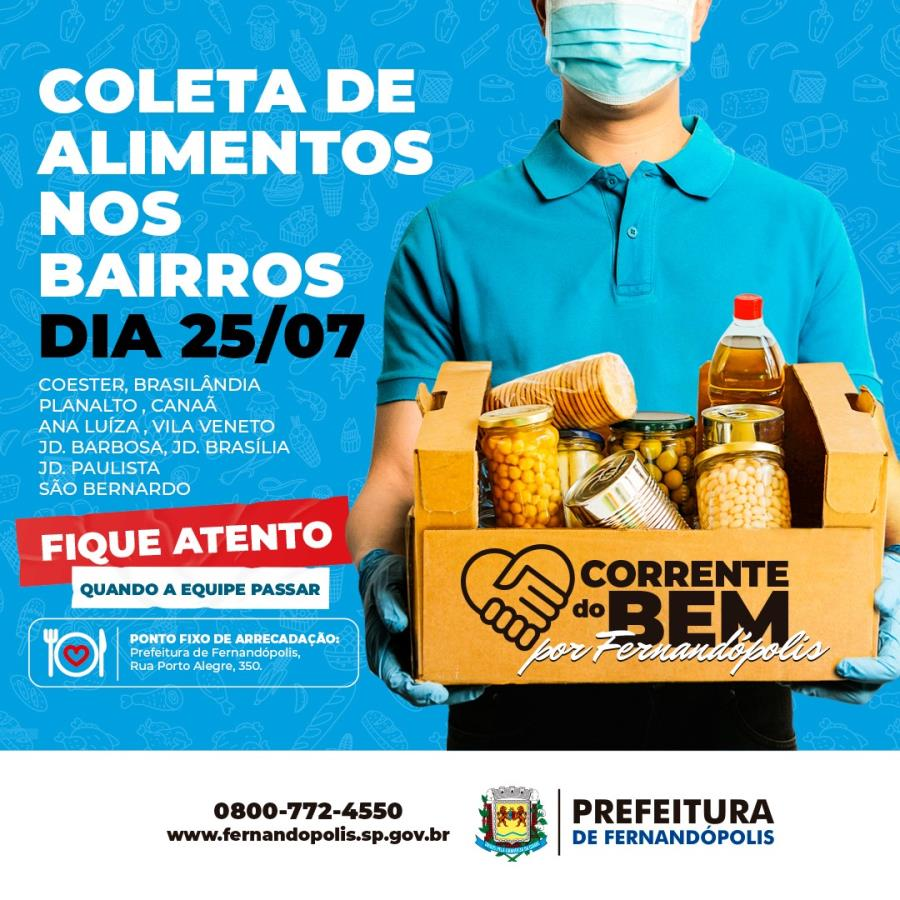
\includegraphics[width=3.71207in,height=3.06667in]{media/image171.jpeg}

%Disponível em:\href{https://fernandopolis.sp.gov.br/campanha-de-arrecadacao-de-alimentos-comeca-no-domingo-dia-25-Acesso\%2011\%20Mar\%202023}{https://fernandopolis.sp.gov.br/campanha-de-arrecadacao-de-alimentos-comeca-no-domingo-dia-25-Acesso 11 mar. 2023}.

Qual é o assunto desse texto?

\begin{escolha}
\item Venda de alimentos.

\item Doação de alimentos.

\item Compra de alimentos.

\item Seleção de alimentos.
\end{escolha}


\num{13} Leia:

\begin{quote}
\textbf{O corvo e o jarro}

Um corvo, quase morto de sede, foi a um jarro, onde pensou encontrar
água. Quando meteu o bico pela borda do jarro, verificou que só havia um
restinho no fundo. Era difícil alcançá-la com o bico, pois o jarro era
muito alto.

Depois de várias tentativas, precisou desistir, desesperado. Surgiu,
então, uma ideia em seu cérebro.

Apanhou um seixo e jogou-o no fundo do jarro. Jogou mais
um e muitos outros.

Com alegria verificou que a água vinha, aos poucos, se aproximando da
borda. Jogou mais alguns seixos e conseguiu matar a sede, salvando a
vida.
\end{quote}

\fonte{Disponível
em: http://www.dominiopublico.gov.br/download/texto/me001614.pdf. Acesso
12 mar. 2023.}

O texto fala da

\begin{escolha}
\item Inteligência do corvo.

\item Tristeza do corvo.

\item Jarro do corvo.

\item Sede do corvo.
\end{escolha}

\num{14} Leia o texto:

\begin{quote}
\textbf{A formiga e a pomba}

Uma formiga sedenta chegou à margem do rio, para beber água. Para alcançar a água, precisou descer por uma folha de grama. Ao fazer isso, escorregou e caiu dentro da correnteza.

Pousada numa árvore próxima, uma pomba viu a formiga em perigo. Rapidamente, arrancou uma folha de árvore e jogou dentro do rio, perto da formiga, que pôde subir nela e flutuar até a margem.
\end{quote}

\fonte{Disponível
em:http://www.dominiopublico.gov.br/download/texto/me001614.pdf. Acesso
em 12 mar. 2023.}

A pomba jogou a folha dentro do rio para

\begin{escolha}
\item Ajudar a formiga.

\item Afogar a formiga.

\item Espantar a formiga.

\item Alimentar a formiga.
\end{escolha}


\num{15} Observe a imagem.

%Paulo: inserir imagem disponível no endereço: https://br.freepik.com/vetores-gratis/homem-com-cara-de-zangado_19714976.htm#query=drawing%20angry%20boy&position=12&from_view=search&track=robertav1_2_sidr

O menino aparenta estar

\begin{escolha}
\item feliz.

\item cansado.

\item bravo.

\item doente.
\end{escolha}

\num{16} Veja o cartaz:

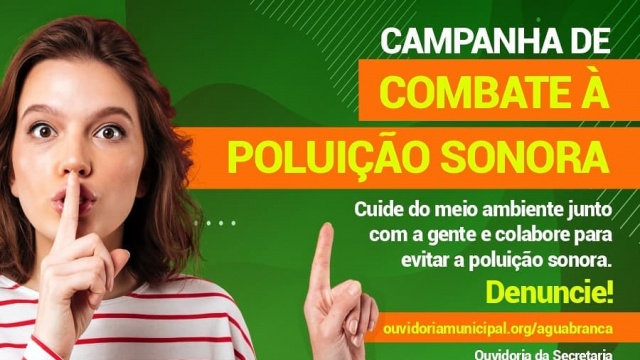
\includegraphics[width=3.64744in,height=2.05233in]{media/image173.png}

%https://aguabranca.pi.gov.br/aguabranca/portalnoticias/noticia/31-12-1969/agua-branca-lanca-campanha-para-combater-a-poluicao-sonora Acesso 11 mar. 2023.

O gesto que a moça está fazendo com a dedo na boca significa

\begin{escolha}
\item calma.

\item silêncio.

\item cuidado.

\item atenção.
\end{escolha}


\chapter{Simulado 4}
\markboth{Simulado 4}{}

\num{1} Veja o animal preferido de Júlia.

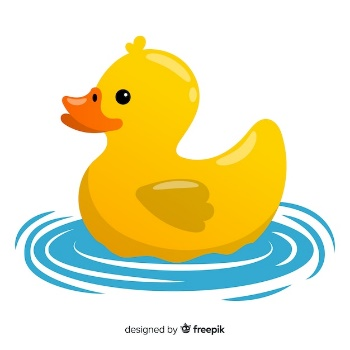
\includegraphics[width=1.58974in,height=1.58974in]{media/image174.jpeg}

%https://www.freepik.com/free-vector/illustration-cute-yellow-rubber-duckling-water\_5422564.htm\#query=PATO\&position=20\&from\_view=search\&track=sph

A palavra cuja letra inicial é igual à do animal preferido de Júlia é

\begin{escolha}
\item Vela.

\item Fafá.

\item Bala.

\item Pipa.
\end{escolha}

\num{2} Esta é a fruta que Mari gosta de levar para o piquinique.

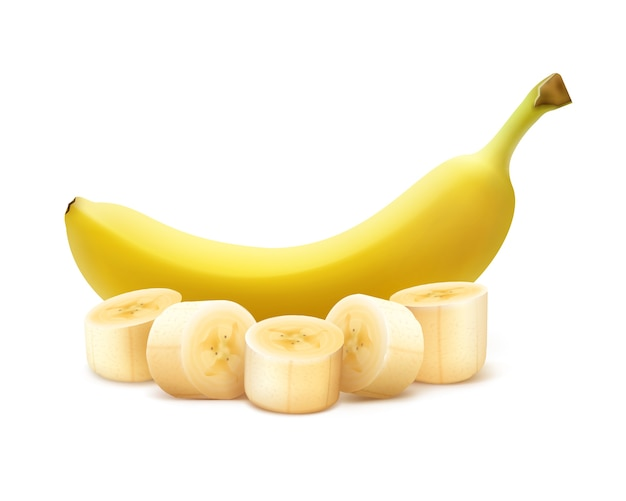
\includegraphics[width=1.96704in,height=1.37153in]{media/image175.jpeg}

%https://www.freepik.com/free-vector/vector-whole-chopped-ripe-yellow-banana-isolated-white-background\_11053227.htm\#query=BANANA\&position=46\&from\_view=search\&track=sph

A sílaba inicial dessa palavra também surge no início de

\begin{escolha}
\item Dado.

\item Bala.

\item Fada.

\item Pato.
\end{escolha}

\num{3} Veja a palavra que Paula escreveu na placa.

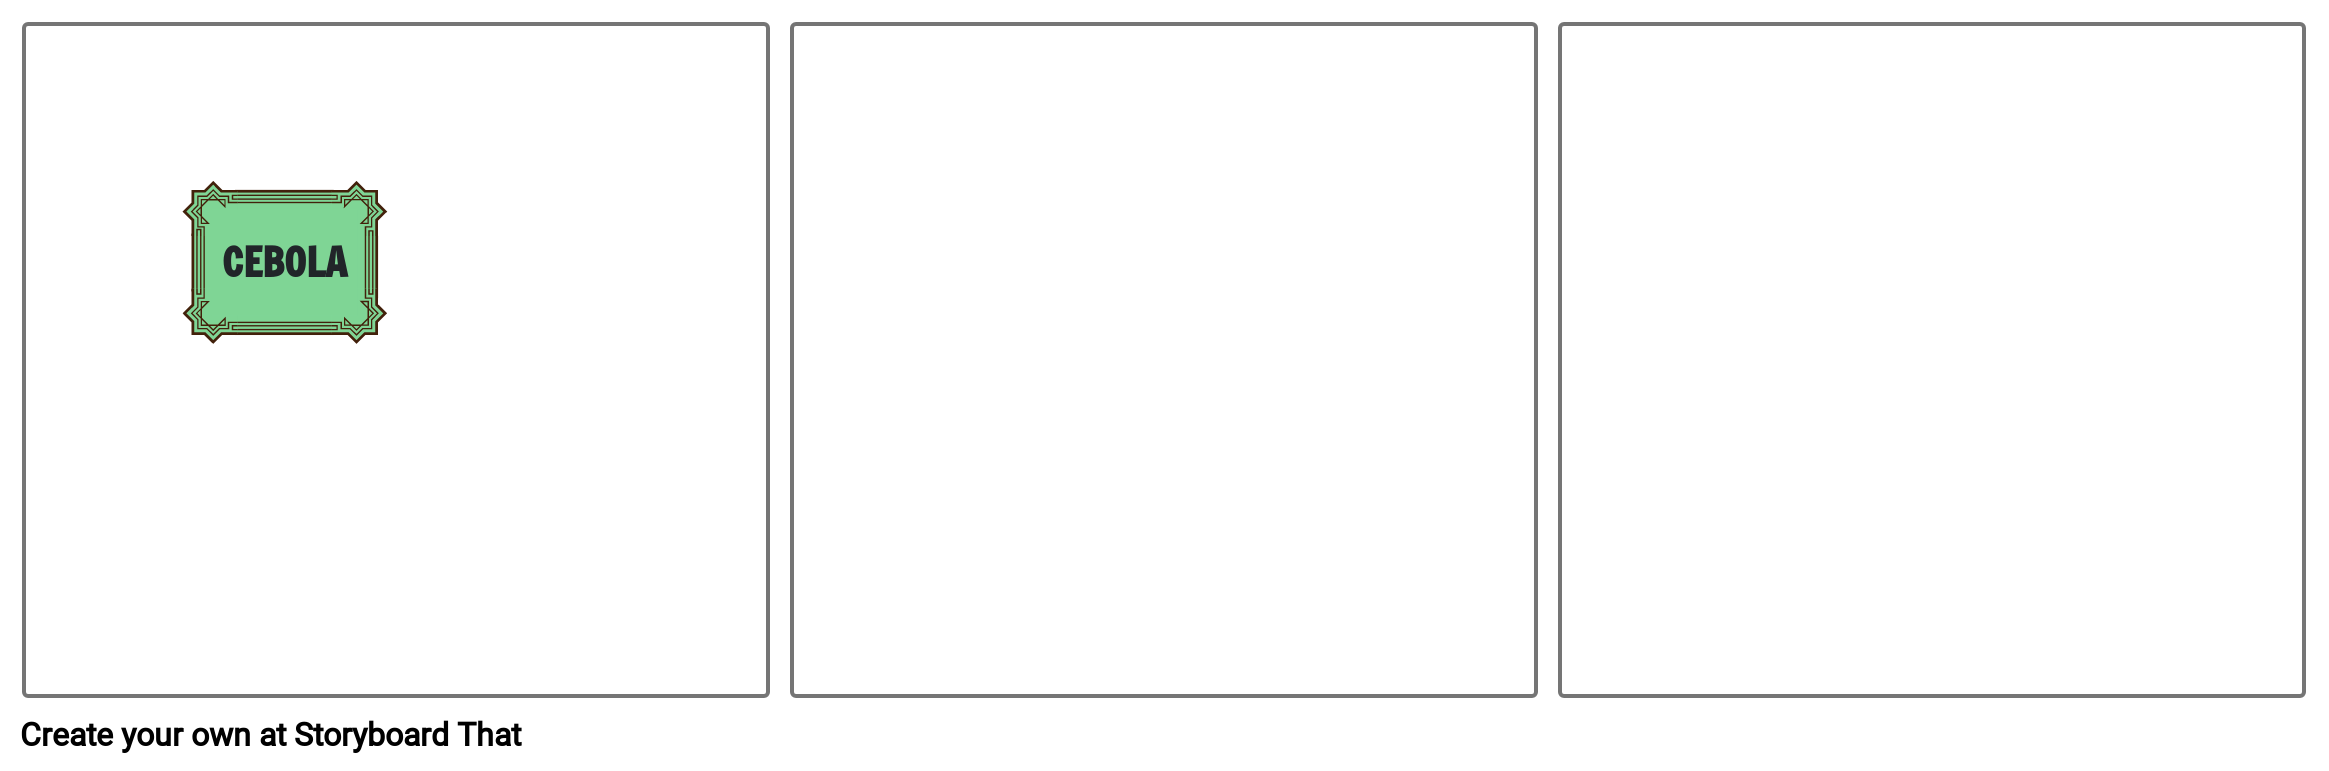
\includegraphics[width=1.19861in,height=1.00625in]{media/image176.png}

%elabodada pela autora

O som da primeira sílaba da palavra também aparece no início de

\begin{escolha}
\item Cinto.

\item Cuscuz.

\item Cegonha.

\item Carroça.
\end{escolha}


\num{4} Veja a palavra que Carla e Maria formaram no alfabeto móvel.

Qual letra pode ser usada para formar uma outra palvara?

\begin{escolha}
\item D

\item P

\item F

\item C
\end{escolha}

\num{5} Veja o brinquedo que Tiago ganhou em uma pescaria.

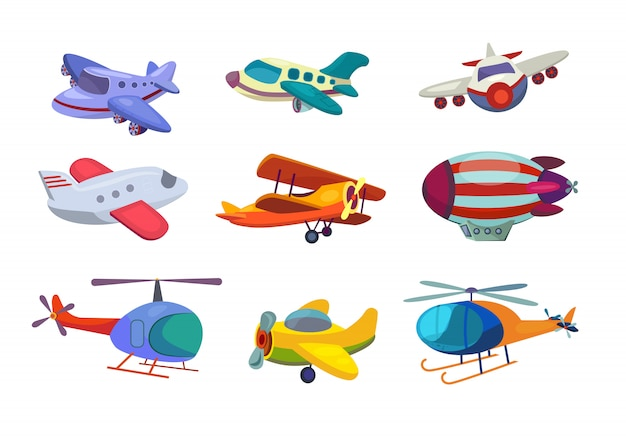
\includegraphics[width=1.69097in,height=0.86538in]{media/image177.jpeg}

%https://www.freepik.com/free-vector/air-transportation-set\_4559015.htm\#query=AVI\%C3\%83O\&position=6\&from\_view=search\&track=sph

Qual palavra é iniciada pela mesma vogal do nome do objeto que Tiago ganhou?

\begin{escolha}
\item Fada.

\item Cravo.

\item Morango.

\item Abacaxi.
\end{escolha}

\num{6} Veja a palavra que Ana escreveu.

%Paulo: Colocar a palavra pedra em um quadro.

A sequência consoante consoante vogal também aparece na sílaba final da palavra

\begin{escolha}
\item Apito.

\item Cravo.

\item Comadre.

\item Escravo.
\end{escolha}

\num{7} Observe o objeto que a tia de Bela pediu para ela comprar.

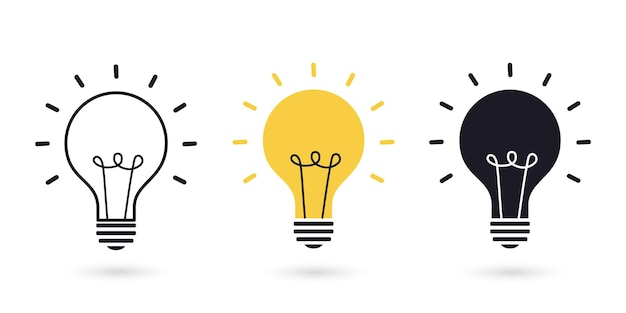
\includegraphics[width=1.07025in,height=1.04487in]{media/image178.jpeg}

%\url{https://www.freepik.com/premium-vector/idea-lamp-icon-line-glyph-filled-outline-colorful-version-abstract-light-bulb-outline-filled_27972598.htm\#query=LAMPADA\&position=15\&from_view=search\&track=sph}

A escrita correta do nome do objeto que Bela comprou é

\begin{escolha}
\item Lâpada.

\item Lâpamda.

\item Lâmpada.

\item Lânpada.
\end{escolha}

\num{8} Observe a imagem.

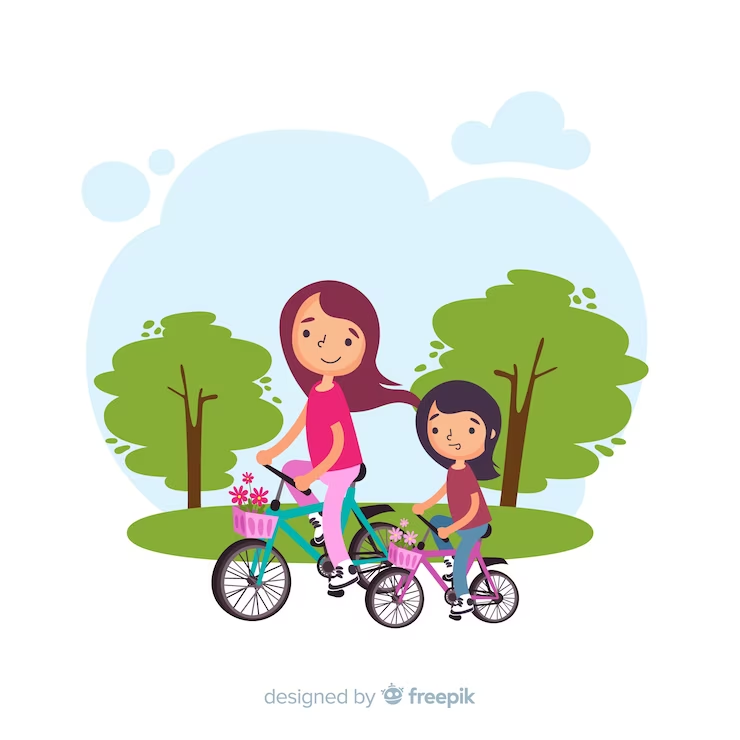
\includegraphics[width=2.76266in,height=1.82051in]{media/image179.png}

%\url{https://www.freepik.com/free-vector/people-riding-bicycles-park_4677113.htm\#query=MENINA\%20DE\%20BICICLETA\&position=16\&from_view=search\&track=ais}

A frase que representa o que está acontecendo na imagem é

\begin{escolha}
\item As meninas caíram de bicicleta.

\item As meninas estão andando de bicicleta.

\item As meninas estão comprando a bicicleta.

\item As meninas estão andando de patinete.
\end{escolha}


\num{9} Veja o presente que Matheus ganhou do seu amigo.

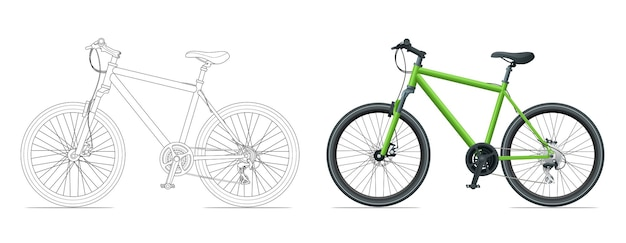
\includegraphics[width=2.46250in,height=1.54444in]{media/image180.jpeg}

%\url{https://www.freepik.com/premium-vector/outline-bicycle-outline-isolated-white-background-mountain-bike-template-moped-motorbike-branding-advertising-vector-illustration_22992461.htm\#query=BICICLETA\&position=6\&from_view=search\&track=sph}

A separação silábica dessa palavra é

\begin{escolha}
\item bi-cicl-eta

\item bici-cle-ta

\item bici-cl-e-ta

\item bi-ci-cle-ta
\end{escolha}

\num{10} Beto, Anita, Caio e Joca estão brincado de bafo.

Veja a quantidade de cartas de cada um.

\begin{longtable}[]{@{}ll@{}}
\toprule
\textbf{CRIANÇAS} & \textbf{QUANTIDADE DE CARTAS}\tabularnewline
\midrule
\endhead
\textbf{BETO} & \textbf{QUATRO}\tabularnewline
\textbf{ANITA} & \textbf{OITO}\tabularnewline
\textbf{CAIO} & \textbf{NOVE}\tabularnewline
\textbf{JOCA} & \textbf{SETE}\tabularnewline
\bottomrule
\end{longtable}

Qual criança tem nove cartas?

\begin{escolha}
\item Joca.

\item Caio.

\item Beto.

\item Anita.
\end{escolha}

\num{11} Leia:

\begin{quote}
\textbf{Surucucu, uma gigante peçonhenta que é especialista em esconde-esconde}

Mesmo com mais de 3 metros de comprimento e habitando todo o Brasil, a
surucucu consegue se esconder muito bem do homem.
\end{quote}

\fonte{https://butantan.gov.br/bubutantan/surucucu-uma-gigante-peconhenta-que-e-especialista-em-esconde-esconde.
Acesso 12 mar. 2023.}

Quem produziu esse texto?

\begin{escolha}
\item Um esportista.

\item Um jornalista.

\item Um bombeiro

\item Um político.
\end{escolha}

\num{12} Observe o cartaz:

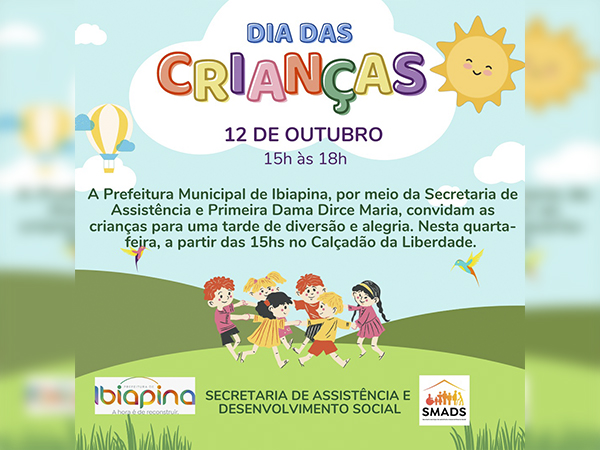
\includegraphics[width=3.22436in,height=2.42060in]{media/image181.jpeg}

%Disponível em:\url{https://ibiapina.ce.gov.br/informa.php?id=1384} Acesso em: 12 mar. 2023.

Esse texto serve para

\begin{escolha}
\item Descrever a festa das crianças.

\item Convidar para a festas das crianças.

\item Ensinar uma bricadeira para as crianças.

\item Falar sobre a situação das crianças no Brasil.
\end{escolha}


\num{13} Leia o texto

\begin{quote}
\textbf{A lebre e a tartaruga.}

Era uma vez... Uma lebre e uma tartaruga.

A lebre vivia caçoando da lerdeza da tartaruga.

Certa vez, a tartaruga, já muito cansada por ser alvo de gozações,
desafiou a lebre para uma corrida.

A lebre, muito segura de si, aceitou prontamente.

Não perdendo tempo, a tartaruga começou a caminhar com seus passinhos
lentos, porém, firmes.

Logo, a lebre ultrapassou a adversária, e vendo que ganharia facilmente, parou
e resolveu cochilar.

Quando acordou, não viu a tartaruga e começou a correr.

Já na reta final, viu finalmente a sua adversária cruzando a linha de
chegada, toda sorridente.
\end{quote}

\fonte{Disponível em: https://pt.wikipedia.org/wiki/A\_Lebre\_e\_a\_Tartaruga.
Acesso 12 mar. 2023. Adaptado.}

A moral dessa história, de acordo com o resultado da corrida, é

\begin{escolha}
\item Não conte vitória antes do tempo.

\item Os mais rápidos sempre vencem.

\item Os fortes conseguem o que querem.

\item As coisas sempre acontecem conforme o esperado.
\end{escolha}


\num{14} Leia o texto:

\begin{quote}
\textbf{A menina das estrelas}

Vanessa estava muito animada no dia do seu aniversário. Passou a tarde
desembrulhando presentes. Uau!! Era um livro. O primeiro livro de
Vanessa. Ela ficou muito curiosa como que poderia estar escrito ali.

Antes de dormir, a mamãe leu o livro para Vanessa. Era sobre uma
garotinha que morava no espaço e tinha seu próprio foguete. Vanessa
ficou encantada. A mãe tinha o costume de olhar o céu pela janela da
casa. Ela começou a juntar coisas que na cabeça dela tinham a ver com o
céu: papel alumínio, pedrinhas, desenhos feitos com tinta guache.
\end{quote}

\fonte{Disponível
em: http://educacao.diadema.sp.gov.br/educacao/attachments/article/660/1o\%20ano.pdf.
Acesso 12 mar. 2023.}

A mãe leu o livro porque Vanessa

\begin{escolha}
\item não sabe ler.

\item gosta de ler.

\item enxerga bem.

\item estava com sono.
\end{escolha}


\num{15}

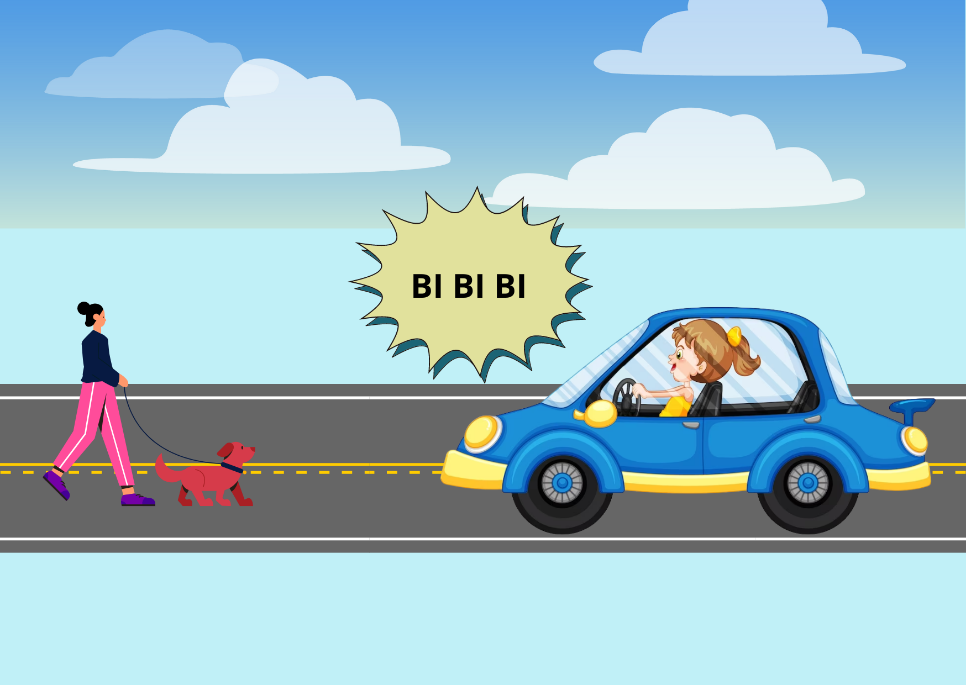
\includegraphics[width=4.38462in,height=3.11119in]{media/image182.png}

%Elaborado pelo autor
%https://www.freepik.com/free-vector/c\%F0\%9F\%98\%81artoon-girl-driving-blue-car\_27180269.htm\#query=MULHER\%20DIRIGINDO\%20CARRO\%20DESENHO\&position=28\&from\_view=search\&track=ais

De acordo com a onomatopeia presente no balão, a mulher está

\begin{escolha}
\item Sorrindo.

\item Gritando.

\item Chorando.

\item Buzinando.
\end{escolha}




